\subsection{可分解线性李代数}

定义 1. 设 g 是 \(\mathfrak{gl}(V)\) 的一个李子代数。称 g 是可分解的，如果 g 含有它的每个元素的半单分量和幂零分量（《代数》，第七章，§5，第 8 节）。

例. 1) 设 \(V'\) 与 \(V''\) 是 V 的向量子空间，满足 \(V'' \supset V'\)。由那些 \(x \in \mathfrak{gl}(V)\)（满足 \(x(V'') \subset V'\)）组成的集是 \(\mathfrak{gl}(V)\) 的一个可分解李子代数；事实上，对所有 \(x \in \mathfrak{gl}(V)\)，x 的半单分量与幂零分量形如 \(P(x)\) 与 \(Q(x)\)，其中 P 与 Q 是没有常数项的多项式。

\begin{enumerate}
\def\labelenumi{\arabic{enumi})}
\setcounter{enumi}{1}
\item
  设 V 具有一个代数结构。V 的导子所成的集是 \(\mathfrak{gl}(V)\) 的一个可分解李子代数（§1，第 1 节，命题 4 (ii)）。
\item
\emph{更一般地，可以证明 \(\mathbf{GL}(\mathrm{V})\) 的任何代数子群的李代数都是可分解的。}
\end{enumerate}

命题 1. 设 \(\mathfrak{g}\) 是 \(\mathfrak{gl}(\mathrm{V})\) 的一个可分解李子代数，\(x \in \mathfrak{g}\)，\(s\) 与 \(n\) 是 \(x\) 的半单分量与幂零分量。

\begin{enumerate}
\def\labelenumi{(\roman{enumi})}
\item
  \(\operatorname{ad}_{\mathfrak{g}}x\) 的半单分量与幂零分量分别是 \(\operatorname{ad}_{\mathfrak{g}}s\) 与 \(\operatorname{ad}_{\mathfrak{g}}n\)。
\item
  \(x\) 在 \(\mathfrak{g}\) 中正则当且仅当 \(s\) 正则。
\item
  若 \(\mathfrak{g}'\) 是 \(\mathfrak{gl}(\mathrm{V})\) 的一个包含 \(\mathfrak{g}\) 的子代数，则 \(\mathfrak{g}\) 的每个初等自同构都可扩张为 \(\mathfrak{g}'\) 的一个初等自同构。
\end{enumerate}

置 \(\mathfrak{a} = \mathfrak{gl}(V)\)。由第一章 §5 第 4 节引理 2，\(\mathrm{ad}_{\mathfrak{a}}x\) 的半单分量与幂零分量是 \(\mathrm{ad}_{\mathfrak{a}}s\) 与 \(\mathrm{ad}_{\mathfrak{a}}n\)；由此得断言 (i)。我们推出 \(\mathrm{ad}_{\mathfrak{g}}x\) 与 \(\mathrm{ad}_{\mathfrak{g}}s\) 的特征多项式相同；故得 (ii)。若 \(\mathrm{ad}_{\mathfrak{g}}x\) 幂零，则 \(\mathrm{ad}_{\mathfrak{g}}x = \mathrm{ad}_{\mathfrak{g}}n\)，于是 \(\mathrm{ad}_{\mathfrak{g}'}n\) 是 \(\mathrm{ad}_{\mathfrak{g}}x\) 的扩张，且 \(n\) 是 \(\mathfrak{g}'\) 的一个幂零元素，故得 (iii)。

设 \(\mathfrak{g}\) 是 \(\mathfrak{gl}(\mathrm{V})\) 的一个李子代数。我们知道（第一章，§6，第 5 节，定理 4），下列条件等价：

\begin{enumerate}
\def\labelenumi{(\roman{enumi})}
\item
  \(\mathfrak{g}\) 的恒等表示是半单的；
\item
  \(\mathfrak{g}\) 是约化的，且 \(\mathfrak{g}\) 的中心的每个元素都是半单自同态。
\end{enumerate}

这些条件实际上等价于下列条件：

\begin{enumerate}
\def\labelenumi{(\roman{enumi})}
\setcounter{enumi}{2}
\tightlist
\item
  \(\mathfrak{g}\) 是 \(\mathfrak{gl}(\mathrm{V})\) 中的一个约化子代数。
\end{enumerate}

事实上，由第一章 §6 第 5 节定理 4 的推论 3 得 (i) \(\Longrightarrow\) (iii)，由第一章 §6 第 6 节命题 7 的推论 1 得 (iii) \(\Longrightarrow\) (i)。我们将证明，若 \(\mathfrak{g}\) 满足这些条件，则 \(\mathfrak{g}\) 是可分解的。更一般地：

命题 2. 设 g 是 \(\mathfrak{gl}(V)\) 的一个李子代数，在 \(\mathfrak{gl}(V)\) 中约化，E 是一个有限维向量空间，\(\pi : g \to \mathfrak{gl}(E)\) 是 g 在 E 上的一个半单线性表示。则：

\begin{enumerate}
\def\labelenumi{(\roman{enumi})}
\item
  \(\mathfrak{g}\) 与 \(\pi (\mathfrak{g})\) 都是可分解的。
\item
  \(\pi(\mathfrak{g})\) 的半单（相应地，幂零）元素是 \(\pi\) 施于 \(\mathfrak{g}\) 的半单（相应地，幂零）元素所得的像。
\item
  若 \(\mathfrak{h}\) 是 \(\mathfrak{gl}(\mathrm{V})\) 的一个包含于 \(\mathfrak{g}\) 的可分解子代数，则 \(\pi(\mathfrak{h})\) 是 \(\mathfrak{gl}(\mathrm{E})\) 的一个可分解子代数。
\item
  若 \(\mathfrak{h}'\) 是 \(\mathfrak{gl}(\mathrm{E})\) 的一个可分解子代数，则 \(\pi^{-1}(\mathfrak{h}')\) 是 \(\mathfrak{gl}(\mathrm{V})\) 的一个可分解子代数。
\end{enumerate}

设 \(\mathfrak{s} = [\mathfrak{g},\mathfrak{g}]\)，并设 \(\mathfrak{c}\) 是 \(\mathfrak{g}\) 的中心。则 \(\mathfrak{g} = \mathfrak{s} \times \mathfrak{c}\)，且由第一章 §6 第 4 节命题 5 的推论，\(\pi(\mathfrak{g}) = \pi(\mathfrak{s}) \times \pi(\mathfrak{c})\)。设 \(y \in \mathfrak{s}, z \in \mathfrak{c}, y_s\) 与 \(y_n\) 是 \(y\) 的半单分量与幂零分量。则 \(y_s, y_n \in \mathfrak{s}\)（第一章，§6，第 3 节，命题 3），\(y_s + z\) 是半单的（《代数》，第七章，§5，第 7 节，命题 16 的推论），且 \(y_n\) 与 \(y_s + z\) 交换。因而 \(y + z\) 的半单分量与幂零分量是 \(y_{s} + z\) 与 \(y_{n}\)。于是 g 是可分解的。由于 \(\pi(\mathfrak{g})\) 在 \(\mathfrak{gl}(\mathrm{E})\) 中约化，同样的论证适用于 \(\pi(\mathfrak{g})\)，并表明 \(\pi(\mathfrak{g})\) 是可分解的。此外，g（相应地，\(\pi(\mathfrak{g})\)）的幂零元素是 s（相应地，\(\pi(\mathfrak{s})\)）的幂零元素。因而 \(\pi(\mathfrak{g})\) 的幂零元素是 \(\pi\) 施于 g 的幂零元素所得的像（第一章，§6，第 3 节，命题 4）。g（相应地，\(\pi(\mathfrak{g})\)）的半单元素是 s（相应地，\(\pi(\mathfrak{s})\)）的半单元素与 c（相应地，\(\pi(\mathfrak{c})\)）的元素之和。于是 \(\pi(\mathfrak{g})\) 的半单元素是 \(\pi\) 施于 g 的半单元素所得的像（第一章，出处同前）。故得 (ii)。

断言 (iii) 与 (iv) 立即由 (i) 与 (ii) 得出。

注记. 1) 对 \(\pi\) 的半单性假定等价于说 \(\pi(x)\) 对所有 \(x \in \mathfrak{c}\) 是半单的。注意，当 \(\pi\) 是由恒等表示 \(\mathfrak{g} \to \mathfrak{gl}(V)\) 相继施行下列运算得到时，这个假定是满足的：张量积，取对偶，取子表示，取商，取直和。

\pandocbounded{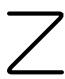
\includegraphics[keepaspectratio]{images/part001_3ab49149.jpg}}

\begin{enumerate}
\def\labelenumi{\arabic{enumi})}
\setcounter{enumi}{1}
\tightlist
\item
  设 \(\mathfrak{g} \subset \mathfrak{gl}(V)\)，\(\mathfrak{g}' \subset \mathfrak{gl}(V')\) 是可分解李代数，\(\varphi\) 是 \(\mathfrak{g}\) 到 \(\mathfrak{g}'\) 的一个同构。注意，\(\varphi\) 未必把 \(\mathfrak{g}\) 的半单（相应地，幂零）元素变为 \(\mathfrak{g}'\) 的半单（相应地，幂零）元素（习题 2）。然而，若 \(\mathfrak{g}\) 半单，则情形就是如此（第一章，§6，第 3 节，定理 3）。
\end{enumerate}

命题 3. 设 \(\mathfrak{a}\) 是 \(\mathfrak{gl}(\mathrm{V})\) 的一个可分解李子代数，并设 \(\mathfrak{b}\) 与 \(\mathfrak{c}\) 是 \(\mathfrak{gl}(\mathrm{V})\) 的向量子空间，满足 \(\mathfrak{b} \subset \mathfrak{c}\)。设 \(\mathfrak{a}'\) 是那些 \(x \in \mathfrak{a}\)（满足 \([x, \mathfrak{c}] \subset \mathfrak{b}\)）所成的集。则 \(\mathfrak{a}'\) 是可分解的。

置 \(\mathfrak{g} = \mathfrak{gl}(\mathrm{V})\)；子代数 \(\mathfrak{h}'\)（\(\mathfrak{gl}(\mathfrak{g})\) 中由那些 \(z \in \mathfrak{gl}(\mathfrak{g})\)（满足 \(z(\mathfrak{c}) \subset \mathfrak{b}\)）组成的）是可分解的（例 1）。设 \(\pi : \mathfrak{g} \to \mathfrak{gl}(\mathfrak{g})\) 是 \(\mathfrak{g}\) 的伴随表示。把命题 2 (iv) 应用于 \(\pi\)，表明 \(\pi^{-1}(\mathfrak{h}')\) 是可分解的。因而 \(\mathfrak{a}' = \mathfrak{a} \cap \pi^{-1}(\mathfrak{h}')\) 也是可分解的。

推论 1. 若 \(\mathfrak{a}\) 是 \(\mathfrak{gl}(\mathrm{V})\) 的一个可分解李子代数，且 \(\mathfrak{n}\) 是 \(\mathfrak{a}\) 的一个李子代数，则 \(\mathfrak{n}\) 在 \(\mathfrak{a}\) 中的正规化子（相应地，中心化子）是可分解的。

这由命题 3 取 \(\mathfrak{c} = \mathfrak{n},\mathfrak{b} = \mathfrak{n}\)（相应地，\(\mathfrak{c} = \mathfrak{n},\mathfrak{b} = \{0\}\)）得到。

推论 2. \(\mathfrak{gl}(\mathrm{V})\) 的一个可分解李子代数的嘉当子代数都是可分解的。

这由推论 1 得出。

注记. 我们将在后面（第 5 节，定理 2）证明推论 2 的一个逆命题。

